\documentclass[11pt]{beamer}
\usetheme{Madrid}

\usepackage[T1]{fontenc}
\usepackage[utf8]{inputenc}
\usepackage{amsmath,amsfonts,amssymb}
\usepackage{graphicx}
\usepackage{xcolor}
\usepackage{tikz}
\usepackage{array}
\usepackage{longtable}
\usepackage{booktabs}

\title{RFE Response Toolkit}
\subtitle{EB2-NIW \& EB1A: Endeavor • 3 Prongs • GenAI • LaTeX}
\author{Strategic RFE Response System}
\date{\today}

\setbeamercovered{transparent}
\setbeamertemplate{navigation symbols}{}

\setbeamerfont{itemize/enumerate body}{size=\scriptsize}
\setbeamerfont{itemize/enumerate subbody}{size=\tiny}
\setbeamerfont{block body}{size=\scriptsize}
\setbeamerfont{block title}{size=\normalsize}

\begin{document}
	
	% TITLE SLIDE
	\begin{frame}
		\titlepage
		\centering
		\scriptsize \textit{Master the Art of RFE Response: EB2-NIW \& EB1A}
	\end{frame}
	
	
	% ============================================================
	% TABLE OF CONTENTS SLIDE - ADD AFTER TITLE SLIDE
	% ============================================================
	
	\begin{frame}{Table of Contents}
		\scriptsize
		\begin{columns}[T]
			\column{0.48\textwidth}
			\textbf{1. Introduction \& Overview}
			\begin{itemize}
				\item What is an RFE?
			RFE vs. NOID vs. Denial
			\end{itemize}
			
			\textbf{2. Analyzing the RFE}
			\begin{itemize}
				\item RFE Notice Key Information
			Missing Form I-140 Sections
				The 3 Prongs of Dhanasar
			\end{itemize}
			
			\textbf{3. Prong 1 - Substantial Merit}
			\begin{itemize}
				\item Common Deficiencies
				\item How to Fix
			\end{itemize}
			
			\textbf{4. Prong 1 - National Importance}
			\begin{itemize}
				\item Common Deficiencies
				How to Fix
			 .gov Evidence Strategy
			\end{itemize}
			
			\textbf{5. Prong 2 - Well-Positioned}
			\begin{itemize}
				\item Common Deficiencies
				How to Fix
			\end{itemize}
			
			\textbf{6. Prong 3 - Balancing Test}
			\begin{itemize}
				\item Common Deficiencies
			 How to Fix
			\end{itemize}
			
			\textbf{7. Expert Opinion Letters}
			\begin{itemize}
				\item What USCIS Looks For
			 Letter Structure Template
			\end{itemize}
			
			\column{0.48\textwidth}
			\textbf{8. Pre-Filing Strategy}
			\begin{itemize}
				\item Work Done Before Filing
				 Documentation Strategy
			Katigbak Distinction
			\end{itemize}
			
			\textbf{9. .gov \& Academic Indexing}
			\begin{itemize}
				\item Science.gov
				 Federal Reserve FEDS
				 EBSCO / Commerce Library
			 Google Scholar \& Semantic Scholar
			ResearchGate \& ORCID
				OSF, RePEc, SSRN, ERIC
			 Harrisburg \& Zuyd University
				ICI \& OUCI
			\end{itemize}
			
			\textbf{10. Open Access Education}
			\begin{itemize}
				\item Udemy Courses
			 Workforce Impact Metrics
			\end{itemize}
			
			\textbf{11. LaTeX \& AI Tools}
			\begin{itemize}
				\item LaTeX for RFE Responses
			 GenAI Prompts (DeepSeek, ChatGPT)
			\end{itemize}
			
			\textbf{12. Post-RFE Options}
			\begin{itemize}
				\item NOID Response
			 I-290B Appeal/Motion
			\end{itemize}
			
			\textbf{13. Paralegal Review \& Checklists}
			\begin{itemize}
				\item Final Checklist
			 Common Mistakes
				Timeline
			\end{itemize}
			
			\textbf{14. Proactive MTR Evidence}
			\begin{itemize}
				\item Awards, Media, International Indexing
			\end{itemize}
		\end{columns}
		\vspace{0.3cm}
		\centering
		\textcolor{blue}{Total Slides: 70+ | Complete RFE Response Toolkit}
	\end{frame}
	% ============================================================
	% SECTION 1: INTRODUCTION & COURSE OVERVIEW
	% ============================================================
	
	\begin{frame}{Course Overview}
		\scriptsize
		\begin{block}{What You Will Learn}
			\begin{itemize}
				\item How to understand and respond to USCIS Requests for Evidence (RFEs)
				\item The 3 Prongs of EB2-NIW under \textit{Matter of Dhanasar}
				\item Using Generative AI (DeepSeek, ChatGPT, Gemini, Perplexity) for RFE responses
				\item LaTeX templates for professional 400+ page applications
				\item Expert opinion letters that address specific RFE concerns
				\item How to prove "Critical Role" for EB1A
				\item Aligning your research with U.S. National Interest
				\item \textcolor{blue}{Analyzing the actual RFE denial notice structure}
			\end{itemize}
		\end{block}
	\end{frame}
	
	\begin{frame}{What is an RFE?}
		\scriptsize
		\begin{block}{Request for Evidence - Definition}
			\textbf{Answer:} An RFE is a formal request from USCIS asking for additional documentation or clarification to determine eligibility.
			\vspace{0.2cm}
			\textbf{Key Facts:}
			\begin{itemize}
				\item Issued when evidence is missing, insufficient, or unclear
				\item Response time: typically 30-87 days
				\item NOT a denial - your case is still alive
				\item Opportunity to strengthen your petition
			\end{itemize}
			\textcolor{red}{Do NOT ignore an RFE. Failure to respond = automatic denial.}
		\end{block}
	\end{frame}
	
	\begin{frame}{RFE vs. NOID vs. Denial}
		\scriptsize
		\begin{block}{Understanding USCIS Actions}
			\centering
			\begin{tabular}{|p{3cm}|p{5cm}|p{2.5cm}|}
				\hline
				\textbf{Action} & \textbf{Meaning} & \textbf{Response Window} \\
				\hline
				RFE & Core eligibility gaps found; case still active & 30-87 days \\
				\hline
				NOID & Intent to deny; serious defects & 30-33 days \\
				\hline
				Denial & Case closed; no further evidence accepted & 30-33 days for appeal \\
				\hline
			\end{tabular}
			\vspace{0.2cm}
			\textcolor{blue}{RFE is the best scenario - you have time to fix the issues.}
		\end{block}
	\end{frame}
	
	% ============================================================
	% SECTION 2: ANALYZING THE RFE STRUCTURE
	% ============================================================
	
	\begin{frame}{The RFE Notice - Key Information (REDACTED)}
		\scriptsize
		\begin{block}{Receipt Details from RFE Notice}
			\textbf{Receipt Number:} [RECEIPT NUMBER]
			\vspace{0.2cm}
			\textbf{Petitioner:} [PETITIONER NAME]
			\vspace{0.2cm}
			\textbf{A-Number:} [A-NUMBER]
			\vspace{0.2cm}
			\textbf{Priority Date:} [DATE]
			\vspace{0.2cm}
			\textbf{Response Deadline:} [DATE]
			\vspace{0.2cm}
			\textbf{Officer:} [OFFICER NAME]
			\vspace{0.2cm}
			\textbf{Service Center:} Texas Service Center (TSC)
		\end{block}
	\end{frame}
	
	\begin{frame}{Missing Information on Form I-140}
		\scriptsize
		\begin{block}{CRITICAL: Form I-140 Deficiencies}
			\textbf{USCIS identified missing information on Form I-140:}
			\vspace{0.2cm}
			\textcolor{red}{\textbf{Part 4 - Processing Information:}} MISSING
			\vspace{0.2cm}
			\textcolor{red}{\textbf{Part 6 - Basic Information About the Proposed Employment:}} MISSING
			\vspace{0.2cm}
			\textbf{Specific fields missing:}
			\begin{itemize}
				\item Job Title
				\item Applicable SOC Code
				\item Nontechnical Job Description
			\end{itemize}
			\textcolor{blue}{ACTION ITEM: Immediately complete missing sections and resubmit with RFE response.}
		\end{block}
	\end{frame}
	
	\begin{frame}{Understanding the 3 Prongs of Dhanasar}
		\scriptsize
		\begin{block}{The Dhanasar Framework (26 I\&N Dec. 884)}
			\textbf{Prong 1:} Proposed endeavor has both substantial merit and national importance
			\vspace{0.2cm}
			\textbf{Prong 2:} Petitioner is well-positioned to advance the proposed endeavor
			\vspace{0.2cm}
			\textbf{Prong 3:} On balance, waiving job offer and labor certification benefits the U.S.
			\vspace{0.2cm}
			\textcolor{red}{The RFE may identify deficiencies in ANY of these three prongs.}
		\end{block}
	\end{frame}
	
	% ============================================================
	% SECTION 3: RFE PRONG 1 - SUBSTANTIAL MERIT
	% ============================================================
	
	\begin{frame}{RFE Prong 1 Deficiency: No Clear Endeavor Description}
		\scriptsize
		\begin{block}{Common USCIS Finding - Substantial Merit}
			\begin{quote}
				``The self-petitioner did not specifically state what position that he intends to propose to do in the United States. A self-petitioner should offer details not only as to what the occupation normally involves, but what types of work the person proposes to undertake specifically within that occupation.''
			\end{quote}
			\textcolor{red}{\textbf{Problem:}} Endeavor is vague - described as generic occupation rather than specific proposed work.
			\vspace{0.2cm}
			\textcolor{blue}{\textbf{Solution:}} Submit a detailed, specific endeavor description with:
			\begin{itemize}
				\item Specific projects and goals
				\item Timeline with milestones
				\item Quantifiable metrics
				\item How this differs from normal job duties
			\end{itemize}
		\end{block}
	\end{frame}
	
	\begin{frame}{How to Fix Prong 1 - Substantial Merit}
		\scriptsize
		\begin{block}{Required Evidence per RFE}
			USCIS specifically requests:
			\begin{itemize}
				\item A detailed description of the proposed endeavor and why it is of substantial merit
				\item Documentary evidence that supports the petitioner's statements
			\end{itemize}
			\textbf{Substantial merit can be shown in:}
			\begin{itemize}
				\item Business, entrepreneurialism, science, technology, culture, health, education
				\item Potential to create significant economic impact
				\item Endeavor related to research or pursuit of knowledge
				\item Potential to create significant cultural impact
			\end{itemize}
		\end{block}
	\end{frame}
	
	% ============================================================
	% SECTION 4: RFE PRONG 1 - NATIONAL IMPORTANCE
	% ============================================================
	
	\begin{frame}{RFE Prong 1 Deficiency: National Importance Not Established}
		\scriptsize
		\begin{block}{Common USCIS Finding - National Importance}
			\begin{quote}
				``The record does not show the self-petitioner has demonstrated a proposed endeavor has broader implications and will operate on such a large scale to impact the U.S. economy. The evidence does not show a proposed endeavor that will increase productivity and profitability of U.S. businesses...''
			\end{quote}
			\textcolor{red}{\textbf{Problem:}} Officer focused on generic industry importance, not your specific endeavor.
			\vspace{0.2cm}
			\textcolor{blue}{\textbf{Key Legal Standard:}} 
			\begin{itemize}
				\item The relevant question is NOT the importance of the field/industry
				\item Focus is on the SPECIFIC endeavor the foreign national proposes to undertake
				\item Endeavor may have national importance even if impact is primarily in one geographic area
			\end{itemize}
		\end{block}
	\end{frame}
	
	\begin{frame}{How to Fix Prong 1 - National Importance}
		\scriptsize
		\begin{block}{Evidence to Demonstrate National Importance}
			\textbf{Submit evidence showing the proposed endeavor:}
			\begin{itemize}
				\item Has national or even global implications within a particular field
				\item Has significant potential to employ U.S. workers
				\item Has other substantial positive economic effects, particularly in economically depressed areas
				\item Will broadly enhance societal welfare or cultural/artistic enrichment
				\item Impacts a matter that a government entity has described as having national importance
			\end{itemize}
			\textbf{Examples of strong evidence:}
			\begin{itemize}
				\item .gov citations (Federal Reserve, Science.gov, ERIC)
				\item Letters from government entities demonstrating interest
				\item Documentation showing work is used across state lines
			\end{itemize}
		\end{block}
	\end{frame}
	
	% ============================================================
	% SECTION 5: RFE PRONG 2 - WELL-POSITIONED
	% ============================================================
	
	\begin{frame}{RFE Prong 2 Deficiency: Not Well-Positioned}
		\scriptsize
		\begin{block}{Common USCIS Finding - Well-Positioned}
			\begin{quote}
				``Not every individual who possesses the necessary educational and professional credentials, skills, and who worked in the field will be found to be well positioned to advance the proposed endeavor. The self-petitioner must go beyond showing expertise in a particular field.''
			\end{quote}
			\textcolor{red}{\textbf{Problem:}} Officer concluded activities are "inherent to the occupation" - normal job duties.
			\vspace{0.2cm}
			\textcolor{blue}{\textbf{Solution:}} Demonstrate your role goes beyond normal expectations:
			\begin{itemize}
				\item Leading, critical, or indispensable role in the endeavor
				\item Progress toward achieving the proposed endeavor
				\item Interest from potential customers, users, or investors
			\end{itemize}
		\end{block}
	\end{frame}
	
	\begin{frame}{How to Fix Prong 2 - Well-Positioned}
		\scriptsize
		\begin{block}{Evidence to Demonstrate Well-Positioned}
			\textbf{Education, skills, knowledge, and record of success:}
			\begin{itemize}
				\item Degrees, certificates, licenses in the field
				\item Patents, trademarks, copyrights owned by petitioner
				\item Letters from experts describing past achievements
				\item Published articles and media reports
				\item Strong citation history documentation
				\item Evidence work has influenced the field
			\end{itemize}
			\textbf{Model or plan for future activities:}
			\begin{itemize}
				\item Detailed plan describing how work will continue in the U.S.
				\item Business model when appropriate
				\item Correspondence from prospective employers/clients
				\item Documentation reflecting feasible plans for financial support
			\end{itemize}
		\end{block}
	\end{frame}
	
	% ============================================================
	% SECTION 6: RFE PRONG 3 - BALANCING TEST
	% ============================================================
	
	\begin{frame}{RFE Prong 3 Deficiency: Balancing Test Not Met}
		\scriptsize
		\begin{block}{Common USCIS Finding - Balancing Test}
			\begin{quote}
				``The letters of support lack specific, detailed information to show, on balance, it would be beneficial to the United States to waive the requirements of a job offer, and thus of a labor certification.''
			\end{quote}
			\textcolor{red}{\textbf{Problem:}} USCIS not persuaded that waiver benefits outweigh labor certification process.
			\vspace{0.2cm}
			\textcolor{blue}{\textbf{Factors USCIS considers:}}
			\begin{itemize}
				\item Whether it would be impractical to secure a job offer or obtain labor certification
				\item Whether U.S. would still benefit even if other qualified U.S. workers are available
				\item Whether national interest is sufficiently urgent to warrant forgoing labor certification
				\item Whether endeavor may lead to potential creation of jobs
				\item Whether self-employed in manner that does not adversely affect U.S. workers
			\end{itemize}
		\end{block}
	\end{frame}
	
	\begin{frame}{How to Fix Prong 3 - Balancing Test}
		\scriptsize
		\begin{block}{Evidence to Demonstrate Balancing Test}
			\textbf{Submit evidence showing:}
			\begin{itemize}
				\item Knowledge or skills are not easily articulated in a labor certification
				\item Benefits to U.S. outweigh those inherent in labor certification process
				\item Letters from interested U.S. government agencies or quasi-governmental entities
				\item Explanation of particular urgency
				\item How U.S. would benefit even if other U.S. workers are available
				\item Why proposed endeavor stands to impact or reduce national shortage
			\end{itemize}
			\textcolor{blue}{The labor certification process is designed to protect domestic labor supply. Your evidence must show why waiving this protection benefits the U.S. despite that purpose.}
		\end{block}
	\end{frame}
	
	% ============================================================
	% SECTION 7: EXPERT OPINION LETTERS
	% ============================================================
	
	\begin{frame}{Expert Opinion Letters - What USCIS Looks For}
		\scriptsize
		\begin{block}{What USCIS Said About Expert Letters}
			\begin{quote}
				``The letters of support lack specific, detailed information to show, on balance, it would be beneficial to the United States to waive the requirements of a job offer... The authors of the letters failed to provide any information how the self-petitioner's work influenced the field or industry and went beyond the self-petitioner's organization.''
			\end{quote}
			\textcolor{red}{\textbf{Problem:}} Generic letters that don't address specific Dhanasar prongs.
			\vspace{0.2cm}
			\textcolor{blue}{\textbf{Solution:}} Each expert letter must:
			\begin{itemize}
				\item Address the SPECIFIC proposed endeavor
				\item Explain how work influences the field BEYOND the employer
				\item Discuss national importance, not just individual qualifications
				\item Include expert's credentials (CV attached)
			\end{itemize}
		\end{block}
	\end{frame}
	
	\begin{frame}{Expert Letter Structure for RFE Response}
		\scriptsize
		\begin{block}{Template for RFE-Focused Expert Letter}
			\textbf{Each expert letter should include:}
			\begin{enumerate}
				\item \textbf{Expert qualifications:} Credentials, experience, publications (resume attached)
				\item \textbf{Relationship to petitioner:} How they know your work (independent review)
				\item \textbf{Understanding of the endeavor:} Restate your proposed work
				\item \textbf{Prong 1 confirmation:} Why the endeavor has national importance (specific, not generic)
				\item \textbf{Prong 2 confirmation:} Why you are well-positioned (beyond normal job duties)
				\item \textbf{Prong 3 confirmation:} Why labor certification waiver benefits the U.S.
				\item \textbf{Specific RFE response:} Directly address officer's concerns
				\item \textbf{Conclusion:} Statement that you meet Dhanasar standards
			\end{enumerate}
			\textcolor{red}{Generic letters are ignored. Letters must address specific RFE language.}
		\end{block}
	\end{frame}
	
	
	
	% ============================================================
	% DETAILED 5-YEAR PLAN SLIDE - FOR PRONG 2 (WELL-POSITIONED)
	% ============================================================
	
	\begin{frame}{Detailed 5-Year Plan - Demonstrating Well-Positioned}
		\scriptsize
		\begin{block}{Why a 5-Year Plan is Critical for RFE Response}
			\textbf{Prong 2 requires showing:}
			\begin{itemize}
				\item A model or plan for future activities
				\item How you intend to continue your work in the United States
				\item Progress toward achieving the proposed endeavor
				\item Feasible plans for financial and operational support
			\end{itemize}
			\textcolor{red}{Without a detailed plan, USCIS cannot conclude you are well-positioned to advance the endeavor.}
		\end{block}
		
		\begin{block}{5-Year Plan Template - Year by Year}
			\centering
			\begin{tabular}{|p{1.5cm}|p{5.5cm}|p{2cm}|}
				\hline
				\textbf{Year} & \textbf{Key Activities \& Milestones} & \textbf{Quantifiable Metric} \\
				\hline
				\textbf{Year 1} & Establish research infrastructure; finalize pending publications; secure collaborations & 3-5 papers submitted; 2 expert collaborations \\
				\hline
				\textbf{Year 2} & Expand research scope; present at major conferences; begin workforce training & 5-7 papers published; 3 conference presentations \\
				\hline
				\textbf{Year 3} & Develop open access educational resources; launch online courses; policy engagement & 2-3 courses launched; 1 policy comment submitted \\
				\hline
				\textbf{Year 4} & Scale workforce training; expand industry partnerships; seek federal recognition & 10,000+ students trained; 2-3 industry partners \\
				\hline
				\textbf{Year 5} & Achieve sustained impact; transition to self-sustaining initiatives; mentor others & 25,000+ cumulative students; research adopted by institutions \\
				\hline
			\end{tabular}
		\end{block}
	\end{frame}
	
	\begin{frame}{5-Year Plan - Research Component}
		\scriptsize
		\begin{block}{Research Timeline \& Publication Goals}
			\textbf{Year 1: Foundation}
			\begin{itemize}
				\item Complete and submit pending manuscripts (3-5 papers)
				\item Establish research collaborations with U.S. institutions
				\item Secure ORCID and Google Scholar profiles for tracking
			\end{itemize}
			\textbf{Year 2: Expansion}
			\begin{itemize}
				\item Publish in peer-reviewed journals (Scopus/WoS indexed)
				\item Present at U.S.-based conferences
				\item Build citation momentum on existing work
			\end{itemize}
			\textbf{Year 3-5: Sustained Impact}
			\begin{itemize}
				\item Maintain publication pipeline (2-3 papers per year)
				\item Achieve cumulative 500+ citations on Google Scholar
				\item Serve as peer reviewer for 5+ journals annually
				\item Mentor junior researchers
			\end{itemize}
			\textcolor{blue}{Each milestone is VERIFIABLE through Google Scholar, ORCID, and journal databases.}
		\end{block}
	\end{frame}
	
	\begin{frame}{5-Year Plan - Workforce Training \& Education}
		\scriptsize
		\begin{block}{Open Access Education Timeline}
			\textbf{Year 1-2: Content Development}
			\begin{itemize}
				\item Develop curriculum for AI/finance/cybersecurity training
				\item Create free online courses (Udemy, YouTube, or institutional platforms)
				\item Target workforce segments: veterans, career changers, professionals
			\end{itemize}
			\textbf{Year 3-4: Launch \& Scale}
			\begin{itemize}
				\item Launch courses with measurable enrollment tracking
				\item Target: 1,000+ students in Year 3; 5,000+ in Year 4
				\item Collect geographic distribution data (nationwide reach)
			\end{itemize}
			\textbf{Year 5: Sustained Impact}
			\begin{itemize}
				\item Achieve 10,000+ cumulative student enrollments
				\item Develop advanced/specialized course offerings
				\item Partner with workforce development organizations
			\end{itemize}
			\textcolor{blue}{Quantifiable metrics: enrollment numbers, completion rates, student feedback.}
		\end{block}
	\end{frame}
	
	\begin{frame}{5-Year Plan - Policy \& Regulatory Engagement}
		\scriptsize
		\begin{block}{Policy Impact Timeline}
			\textbf{Ongoing (Years 1-5):}
			\begin{itemize}
				\item Monitor Regulations.gov for relevant RFIs/NPRMs
				\item Submit research-backed policy comments (2-3 per year)
				\item Track citations of comments in final rules
			\end{itemize}
			\textbf{Year 2-3: Government Recognition Goals}
			\begin{itemize}
				\item Seek citation by Federal Reserve, Science.gov, or ERIC
				\item Engage with professional organizations for endorsements
				\item Build portfolio of .gov citations
			\end{itemize}
			\textbf{Year 4-5: Thought Leadership}
			\begin{itemize}
				\item Participate in industry working groups
				\item Contribute to policy white papers
				\item Establish reputation as subject matter expert
			\end{itemize}
			\textcolor{blue}{Policy engagement directly supports Prong 1 (national importance) and Prong 3 (balancing test).}
		\end{block}
	\end{frame}
	
	\begin{frame}{5-Year Plan - Industry Collaboration \& Partnerships}
		\scriptsize
		\begin{block}{Building Industry Relationships}
			\textbf{Year 1:}
			\begin{itemize}
				\item Identify potential industry partners (banks, tech companies, training organizations)
				\item Leverage existing professional network
			\end{itemize}
			\textbf{Year 2-3:}
			\begin{itemize}
				\item Formalize 2-3 collaboration agreements
				\item Provide consulting or advisory services
				\item Document industry adoption of methodologies
			\end{itemize}
			\textbf{Year 4-5:}
			\begin{itemize}
				\item Expand to 5+ industry partnerships
				\item Secure letters of support for immigration purposes
				\item Demonstrate real-world impact of research
			\end{itemize}
			\textcolor{blue}{Industry testimonials and EVL (Employer Verification Letters) are powerful Prong 3 evidence.}
		\end{block}
	\end{frame}
	
	\begin{frame}{5-Year Plan - Quantifiable Metrics Summary}
		\scriptsize
		\begin{block}{Measurable Outcomes by Year 5}
			\centering
			\begin{tabular}{|p{4cm}|p{5cm}|}
				\hline
				\textbf{Category} & \textbf{Target Metric} \\
				\hline
				Peer-reviewed publications & 15-20 total papers \\
				\hline
				Google Scholar citations & 500+ \\
				\hline
				h-index & 10+ \\
				\hline
				Peer review credits & 20+ reviews (WoS/ORCID) \\
				\hline
				Open access students trained & 10,000+ \\
				\hline
				Policy comments submitted & 10-15 \\
				\hline
				.gov citations & 3-5 (Federal Reserve, Science.gov, ERIC) \\
				\hline
				Industry partnerships & 3-5 \\
				\hline
				Conference presentations & 5-7 \\
				\hline
			\end{tabular}
		\end{block}
	\end{frame}
	
	\begin{frame}{How to Present 5-Year Plan in RFE Response}
		\scriptsize
		\begin{block}{Sample Language for RFE Response}
			\begin{quote}
				``Petitioner submits the following 5-Year Plan demonstrating he is well-positioned to advance the proposed endeavor:
				
				\textbf{Year 1:} Complete pending publications (Exhibits A-C). Establish research collaborations with [INSTITUTIONS].
				
				\textbf{Year 2:} Publish 5-7 peer-reviewed papers in Scopus/WoS journals (Exhibit D). Present at [CONFERENCES].
				
				\textbf{Year 3:} Launch open access workforce training courses targeting U.S. veterans and career changers. Target 1,000+ enrollments.
				
				\textbf{Year 4:} Scale training to 5,000+ students nationwide. Expand industry partnerships.
				
				\textbf{Year 5:} Achieve 10,000+ cumulative students, 500+ citations, and sustained research output.
				
				Each milestone is VERIFIABLE through:
				- Publication records (Google Scholar, ORCID, Scopus)
				- Enrollment dashboards (Udemy/institutional platforms)
				- Citation tracking (Google Scholar, Semantic Scholar)
				- Policy comments (Regulations.gov docket numbers)''
			\end{quote}
		\end{block}
	\end{frame}
	
	\begin{frame}{Connecting 5-Year Plan to Katigbak Strategy}
		\scriptsize
		\begin{block}{Why This Plan is NOT a Post-Filing Achievement}
			\textbf{What USCIS may incorrectly argue:}
			\begin{quote}
				``The 5-year plan describes FUTURE work, so it cannot support eligibility at filing.''
			\end{quote}
			\textbf{Your counter-argument:}
			\begin{quote}
				``The 5-year plan demonstrates that the Petitioner HAD a concrete, detailed plan at the time of filing - not that future achievements create new eligibility. Under \textit{Matter of Dhanasar}, the national importance inquiry is PROSPECTIVE (focused on future impact). A detailed plan showing HOW the endeavor will be executed is precisely what Prong 2 requires.''
			\end{quote}
			\textbf{Supporting evidence:}
			\begin{itemize}
				\item Include timestamps showing plan was created BEFORE filing
				\item Reference specific sections of original petition that outlined this plan
				\item Show that Year 1 activities are already underway (pre-filing)
			\end{itemize}
			\textcolor{green}{A detailed 5-year plan with verifiable metrics is STRONG evidence for Prong 2.}
		\end{block}
	\end{frame}
	
	\begin{frame}{5-Year Plan - Evidence Checklist for RFE}
		\scriptsize
		\begin{block}{Before Submitting, Ensure You Have:}
			\begin{itemize}
				\item [$\square$] Written 5-year plan with annual milestones (1-2 pages)
				\item [$\square$] Specific, quantifiable metrics for each year
				\item [$\square$] Timeline showing plan was created BEFORE filing date
				\item [$\square$] Reference to original petition where plan was described
				\item [$\square$] Evidence that Year 1 activities are already in progress
				\item [$\square$] Connection between plan and each Dhanasar prong
				\item [$\square$] Supporting documentation for each milestone type:
				\begin{itemize}
					\item Publications - journal submission receipts, DOIs
					\item Training - platform screenshots, enrollment data
					\item Policy - Regulations.gov submission confirmations
					\item Industry - collaboration letters, EVLs
				\end{itemize}
			\end{itemize}
			\textcolor{blue}{A well-documented 5-year plan is often the DIFFERENCE between approval and denial.}
		\end{block}
	\end{frame}
	
	
	
	% ============================================================
	% HANDLING RFE CLAIMING ENDEAVOR CHANGED - SAME ENDEAVOR, MORE DETAIL
	% ============================================================
	
	\begin{frame}{Handling RFE Claims That Endeavor "Changed"}
		\scriptsize
		\begin{block}{The Problem - USCIS May Claim Endeavor Changed}
			\textbf{Common RFE Trap:}
			\begin{quote}
				``The petitioner's RFE response describes a different endeavor than what was originally proposed. The endeavor has changed, and USCIS cannot evaluate eligibility based on a new endeavor.''
			\end{quote}
			\textcolor{red}{USCIS uses this argument to deny without reviewing the merits of your response.}
			\vspace{0.2cm}
			\textbf{The Truth:}
			\begin{itemize}
				\item The endeavor is the SAME as originally proposed
				\item Your RFE response provides GREATER DETAIL and CLARIFICATION
				\item Greater detail does NOT equal a change in endeavor
				\item Adding specificity, timelines, and metrics is CLARIFICATION, not change
			\end{itemize}
		\end{block}
	\end{frame}
	
	\begin{frame}{Legal Argument: Clarification vs. Change}
		\scriptsize
		\begin{block}{What the Law Says}
			\textbf{Key Principle:} Providing additional detail about an existing endeavor is NOT a change.
			\vspace{0.2cm}
			\textbf{Examples:}
			\begin{tabular}{|p{5cm}|p{5cm}|}
				\hline
				\textbf{NOT a Change (Permissible)} & \textbf{Actual Change (Not Permissible)} \\
				\hline
				Adding specific project names & Switching to completely different field \\
				\hline
				Including timeline with milestones & Changing from research to business \\
				\hline
				Naming specific collaborators & Changing target beneficiaries \\
				\hline
				Quantifying expected outcomes & Abandoning original endeavor entirely \\
				\hline
				Clarifying methods and approaches & Proposing entirely new activities \\
				\hline
			\end{tabular}
			\vspace{0.2cm}
			\textcolor{blue}{The original petition said ``I will do research on AI in finance.'' The RFE response adds ``I will publish 5 papers, train 10,000 students, and collaborate with X institution.'' This is CLARIFICATION, not change.}
		\end{block}
	\end{frame}
	
	\begin{frame}{How to Structure RFE Response to Avoid "Change" Argument}
		\scriptsize
		\begin{block}{Strategy: Explicitly Reference Original Petition}
			\textbf{In your RFE response, include language like:}
			\vspace{0.2cm}
			\begin{quote}
				``This response does NOT propose a new or different endeavor. Rather, it provides the GREATER DETAIL and SPECIFICITY that the original RFE requested.
				
				As stated in the original petition filed on [DATE], Petitioner proposed to [QUOTE ORIGINAL ENDEAVOR LANGUAGE].
				
				The tables, timelines, and metrics below simply ELABORATE on the same endeavor by:
				- Adding specific milestones to the existing timeline
				- Quantifying the expected outcomes originally described
				- Naming specific collaborators and institutions
				- Providing verifiable metrics for the originally stated goals
				
				The core endeavor remains IDENTICAL to what was originally proposed. No new activities have been added. Only the level of detail has increased.''
			\end{quote}
		\end{block}
	\end{frame}
	
	\begin{frame}{Visual: Endeavor Detail vs. Endeavor Change}
		\scriptsize
		\begin{center}
			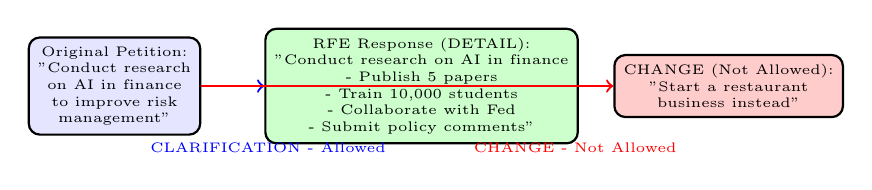
\begin{tikzpicture}[scale=0.65, every node/.style={draw, rounded corners, align=center, font=\tiny}]
				\node (original) at (0,0) [fill=blue!10, draw=black, thick] {Original Petition:\\"Conduct research\\on AI in finance\\to improve risk\\management"};
				\node (detail) at (6,0) [fill=green!20, draw=black, thick] {RFE Response (DETAIL):\\"Conduct research on AI in finance\\- Publish 5 papers\\- Train 10,000 students\\- Collaborate with Fed\\- Submit policy comments"};
				\node (change) at (12,0) [fill=red!20, draw=black, thick] {CHANGE (Not Allowed):\\"Start a restaurant\\business instead"};
				\draw[->, thick, blue] (original) -- (detail);
				\draw[->, thick, red] (original) -- (change);
				\node at (3,-1.2) [draw=none, blue] {CLARIFICATION - Allowed};
				\node at (9,-1.2) [draw=none, red] {CHANGE - Not Allowed};
			\end{tikzpicture}
		\end{center}
	\end{frame}
	
	\begin{frame}{Pre-Emptive Language to Block "Change" Argument}
		\scriptsize
		\begin{block}{Include This Language in Your RFE Response}
			\begin{quote}
				\textbf{At the beginning of your response:}
				
				``Petitioner respectfully submits that this response in no way alters or changes the proposed endeavor as originally described in the Form I-140 petition filed on [DATE]. The original petition stated: [QUOTE].
				
				The additional details, timelines, metrics, and supporting documentation provided herein serve only to ELABORATE, CLARIFY, and provide EVIDENCE in support of the SAME endeavor. USCIS's RFE specifically requested greater specificity regarding the proposed endeavor. This response provides that specificity.
				
				Any suggestion that providing greater detail constitutes a change in endeavor would penalize petitioners for responding to RFEs as requested, which cannot be the intent of the regulations.''
			\end{quote}
			\textcolor{blue}{This language creates a record that you are NOT changing your endeavor.}
		\end{block}
	\end{frame}
	
	\begin{frame}{Case Law Support - Clarification is Permissible}
		\scriptsize
		\begin{block}{Matter of Katigbak - Key Distinction}
			\textbf{What Katigbak prohibits:}
			\begin{itemize}
				\item Brand new evidence of achievements that did NOT exist at filing
				\item Fundamentally different endeavor than originally proposed
			\end{itemize}
			\textbf{What Katigbak does NOT prohibit:}
			\begin{itemize}
				\item Clarification of facts that existed at the time of filing
				\item Additional detail about the SAME endeavor
				\item Evidence that corroborates the originally stated goals
			\end{itemize}
			\textcolor{blue}{Adding a 5-year plan with milestones is CLARIFICATION of the existing endeavor, not creation of a new one.}
			\vspace{0.2cm}
			\textbf{See also:}
			\begin{itemize}
				\item \textit{Matter of Chawathe} - preponderance of evidence standard
				\item \textit{Matter of Dhanasar} - prospective impact inquiry
			\end{itemize}
		\end{block}
	\end{frame}
	
	\begin{frame}{How USCIS Might Argue "Change" - And Your Rebuttal}
		\scriptsize
		\begin{block}{Potential USCIS Argument \#1}
			\textbf{USCIS:} ``The RFE response describes training programs not mentioned in the original petition.''
			\vspace{0.1cm}
			\textbf{Rebuttal:} ``The original petition stated Petitioner would 'enhance workforce skills.' The RFE response specifies that this will be accomplished through open access courses. This is SPECIFICATION, not addition.''
		\end{block}
		\begin{block}{Potential USCIS Argument \#2}
			\textbf{USCIS:} ``The RFE response includes collaboration with specific institutions not named before.''
			\vspace{0.1cm}
			\textbf{Rebuttal:} ``The original petition stated Petitioner would 'collaborate with industry partners.' The RFE response names specific partners as examples of the TYPE of collaboration contemplated. The endeavor remains unchanged.''
		\end{block}
		\begin{block}{Potential USCIS Argument \#3}
			\textbf{USCIS:} ``The RFE response adds quantifiable metrics that were not in the original.''
			\vspace{0.1cm}
			\textbf{Rebuttal:} ``The RFE specifically requested 'quantifiable metrics' and 'evidence of prospective impact.' Providing what was requested is not a change in endeavor - it is compliance with the RFE.''
		\end{block}
	\end{frame}
	
	\begin{frame}{Practical Tips to Avoid "Change" Argument}
		\scriptsize
		\begin{block}{Do This - Safe Approach}
			\begin{itemize}
				\item [$\checkmark$] Quote the original endeavor verbatim at the start of your response
				\item [$\checkmark$] Use phrases like ``to clarify,'' ``to elaborate,'' ``to provide specificity''
				\item [$\checkmark$] Explicitly state ``This is the SAME endeavor as originally proposed''
				\item [$\checkmark$] Organize response as elaboration of original categories
				\item [$\checkmark$] Keep the core description identical; add details as subsections
			\end{itemize}
		\end{block}
		\begin{block}{Do NOT Do This - Risky Approach}
			\begin{itemize}
				\item [$\times$] Rewrite the endeavor description in completely new language
				\item [$\times$] Add entirely new categories of activity not implied in original
				\item [$\times$] Remove or abandon elements of the original endeavor
				\item [$\times$] Use phrases like ``I now propose to...''
				\item [$\times$] Submit response without referencing the original petition language
			\end{itemize}
		\end{block}
	\end{frame}
	
	\begin{frame}{Sample Side-by-Side - Original vs. RFE Response}
		\scriptsize
		\begin{block}{Original Petition Endeavor Description}
			\begin{quote}
				``I propose to continue my research on AI-driven financial risk modeling, focusing on developing open-source tools for community banks and credit unions to detect fraud and ensure regulatory compliance. This endeavor will enhance financial stability across the U.S. banking system.''
			\end{quote}
		\end{block}
		\begin{block}{RFE Response (SAME Endeavor, MORE Detail)}
			\begin{quote}
				``Petitioner reaffirms the SAME proposed endeavor as originally described: research on AI-driven financial risk modeling for community banks and credit unions.
				
				To provide the specificity requested in the RFE, Petitioner adds:
				- A 5-year publication plan targeting 5-7 papers in Scopus/WoS journals
				- A workforce training initiative targeting 10,000+ community bank employees
				- Collaboration with [INSTITUTION] for research validation
				- Policy comments submitted to [AGENCY] on relevant regulations
				
				All of these activities are DIRECTLY DERIVED from the original endeavor description and represent ELABORATION, not change.''
			\end{quote}
		\end{block}
	\end{frame}
	
	\begin{frame}{Final Checklist - Avoiding "Endeavor Changed" RFE Trap}
		\scriptsize
		\begin{block}{Before Submitting RFE Response, Verify:}
			\begin{itemize}
				\item [$\square$] Original endeavor quoted verbatim in the response
				\item [$\square$] Explicit statement that endeavor has NOT changed
				\item [$\square$] New details are clearly linked to original categories
				\item [$\square$] No categories of activity removed from original
				\item [$\square$] No completely new categories added (only specified existing ones)
				\item [$\square$] Response uses language of CLARIFICATION, not CHANGE
			\item [$\square$] Original petition referenced throughout (page numbers, exhibit references)
			\item [$\square$] Legal citations ready to counter "change" argument (Katigbak, Chawathe)
		\end{itemize}
		\textcolor{blue}{The goal: Make it IMPOSSIBLE for USCIS to claim the endeavor changed without misrepresenting your response.}
		\vspace{0.2cm}
		\textcolor{red}{Remember: Greater detail = Clarification. Clarification = Permissible. Change = Not permissible. Your response must be the former.}
	\end{block}
	\end{frame}
	% ============================================================
	% SECTION 8: THE PRE-FILING STRATEGY
	% ============================================================
	
	\begin{frame}{The Pre-Filing Strategy: Work Done Before Filing}
		\scriptsize
		\begin{block}{Key Argument: Pending Publications and Work in Progress}
			\textbf{The Problem with RFEs:}
			\begin{itemize}
				\item USCIS often demands evidence of "already achieved" impact
				\item But the NIW standard is PROSPECTIVE (\textit{Dhanasar})
				\item Officers confuse EB-1A (past achievements) with EB2-NIW (future potential)
			\end{itemize}
			\textbf{The Strategic Answer:}
			\begin{itemize}
				\item \textcolor{blue}{Show that work was ALREADY IN PROGRESS before filing}
				\item \textcolor{blue}{Pending publications count as "work done" not "new achievements"}
				\item \textcolor{blue}{The research was ongoing - not started after filing}
			\end{itemize}
		\end{block}
	\end{frame}
	
	\begin{frame}{"The Work Was Already Told" - Documentation Strategy}
		\scriptsize
		\begin{block}{Proving Pre-Filing Work Existed}
			\textbf{What you need to show:}
			\begin{itemize}
				\item The original petition mentioned the research direction
				\item Draft manuscripts existed BEFORE the filing date
				\item Preprints were submitted to preprint servers before filing
				\item Research collaborations were established before filing
				\item Data collection was completed before filing
			\end{itemize}
			\textbf{How to prove it:}
			\begin{itemize}
				\item Email timestamps showing manuscript drafts
				\item Submission receipts from preprint servers (dated before filing)
				\item Version control history showing pre-filing work
				\item Expert letters confirming the work was underway
			\end{itemize}
			\textcolor{red}{If you can prove work was ongoing, it is NOT a post-filing achievement.}
		\end{block}
	\end{frame}
	
	\begin{frame}{Pending Publications Are NOT Post-Filing Achievements}
		\scriptsize
		\begin{block}{The Key Distinction Under Matter of Katigbak}
			\textbf{Katigbak bars:}
			\begin{itemize}
				\item New papers published AFTER the filing date
				\item New awards received AFTER the filing date
				\item New citations earned AFTER the filing date
			\end{itemize}
			\textbf{Katigbak does NOT bar:}
			\begin{itemize}
				\item \textcolor{green}{Papers that were SUBMITTED before filing (even if published later)}
				\item \textcolor{green}{Research that was IN PROGRESS at time of filing}
				\item \textcolor{green}{Work that was "already told" in the original petition}
			\end{itemize}
			\textbf{Strategic argument:}
			\begin{quote}
				``The pending publications represent the natural fruition of work that was already described, in progress, and ongoing at the time of filing. They do not create new eligibility; they merely confirm the viability and execution of the originally proposed endeavor.''
			\end{quote}
		\end{block}
	\end{frame}
	
	% ============================================================
	% SECTION 9: .GOV INDEXING STRATEGY
	% ============================================================
	
	\begin{frame}{Using .gov Indexing as RFE Evidence}
		\scriptsize
		\begin{block}{Science.gov Indexing - Federal Recognition}
			\textbf{What is Science.gov?}
			\begin{itemize}
				\item Official U.S. government portal for scientific information
				\item Searches 60+ federal databases
				\item Indexing means federal agencies found your work valuable
			\end{itemize}
			\textbf{Why this matters for RFE:}
			\begin{itemize}
				\item Direct .gov domain evidence of national importance
				\item Verifiable by USCIS through science.gov
				\item Shows your research is used by U.S. government scientists
				\item Counts as "professional recognition" for EB1A
			\end{itemize}
			\textcolor{blue}{Having your papers indexed on Science.gov is objective proof that federal agencies consider your work valuable.}
		\end{block}
	\end{frame}
	
	\begin{frame}{Federal Reserve FEDS Series Citation}
		\scriptsize
		\begin{block}{Finance and Economics Discussion Series (FEDS)}
			\textbf{What is FEDS?}
			\begin{itemize}
				\item Official publication of the Federal Reserve Board
				\item Peer-reviewed research on U.S. financial and economic policy
				\item Widely used by policymakers, researchers, and financial institutions
			\end{itemize}
			\textbf{Why this is powerful RFE evidence:}
			\begin{itemize}
				\item Direct citation by the U.S. central bank
				\item Proves your research influences federal policy
				\item Uniquely strong evidence for Prong 1 (national importance)
				\item Cannot be dismissed as "insufficient" without explanation
			\end{itemize}
			\textcolor{red}{A Federal Reserve citation is among the strongest possible evidence for NIW.}
		\end{block}
	\end{frame}
	
	\begin{frame}{EBSCO and U.S. Commerce Library Indexing}
		\scriptsize
		\begin{block}{Getting Indexed in U.S. Commerce Research Library}
			\textbf{What is the Commerce Research Library?}
			\begin{itemize}
				\item Official library of the U.S. Department of Commerce
				\item Indexes journals through EBSCO Business Source Complete
				\item Your work becomes searchable by Commerce Department policymakers
			\end{itemize}
			\textbf{Why this matters:}
			\begin{itemize}
				\item Direct .gov indexing through EBSCO
				\item Accessible to U.S. trade and economic policymakers
				\item Demonstrates relevance to U.S. commercial and economic policy
				\item Verifiable by USCIS through search.library.doc.gov
			\end{itemize}
			\textcolor{blue}{EBSCO indexing through Commerce Library = .gov recognition for business research.}
		\end{block}
	\end{frame}
	
	% ============================================================
	% SECTION 10: OPEN ACCESS EDUCATION EVIDENCE
	% ============================================================
	
	\begin{frame}{Udemy Courses and Open Access Education}
		\scriptsize
		\begin{block}{Demonstrating Workforce Impact Through Open Education}
			\textbf{What to include in RFE response:}
			\begin{itemize}
				\item Screenshots of course enrollments (online learning platforms)
				\item Number of students trained (quantifiable metric)
				\item Geographic distribution of students (nationwide reach)
				\item Free/open access courses (demonstrates public service)
			\end{itemize}
			\textbf{Why this matters for Prong 1:}
			\begin{itemize}
				\item Shows direct impact on U.S. workforce development
				\item Quantifiable metrics (e.g., "thousands of students trained")
				\item Demonstrates broader implications beyond employer
				\item Particularly valuable for retraining/upskilling endeavors
			\end{itemize}
			\textcolor{blue}{Open access education metrics are objective evidence of nationwide impact.}
		\end{block}
	\end{frame}
	
	% ============================================================
	% SECTION 11: USING LATEX FOR RFE RESPONSES
	% ============================================================
	
	\begin{frame}{Why Use LaTeX for RFE Responses}
		\scriptsize
		\begin{block}{LaTeX Advantages for Immigration Filings}
			\textbf{Benefits:}
			\begin{itemize}
				\item Professional formatting (law-firm quality)
				\item Automatic table of contents and cross-references
				\item Consistent exhibit numbering
				\item Easy to update and version control
				\item Handles 400+ page documents seamlessly
				\item Free (Overleaf, TeX Live)
			\end{itemize}
			\textbf{What to templatize:}
			\begin{itemize}
				\item RFE response briefs
				\item Covering letters addressing each deficiency
				\item Exhibit indexes and organization
				\item Expert opinion letters
			\end{itemize}
		\end{block}
	\end{frame}
	
	\begin{frame}{LaTeX RFE Response Structure}
		\scriptsize
		\begin{block}{Organizing Your RFE Response in LaTeX}
			\begin{enumerate}
				\item \textbf{Main file (master\_rfe.tex):} \texttt{\textbackslash input} for each section
				\item \textbf{Cover letter (covering.tex):} Executive summary addressing each RFE point
				\item \textbf{Response to each deficiency:} Separate section per RFE issue
				\item \textbf{Exhibits:} Organized as Exhibit A, B, C...
				\item \textbf{Expert letters:} Individual files \texttt{\textbackslash input}
				\item \textbf{Evidence tables:} Publications, citations, peer reviews
			\end{enumerate}
			\textcolor{blue}{Use \texttt{\textbackslash includeonly} to test specific sections while compiling.}
		\end{block}
	\end{frame}
	
	% ============================================================
	% SECTION 12: GENERATIVE AI FOR RFE RESPONSES
	% ============================================================
	
	\begin{frame}{GenAI Tools for RFE Responses}
		\scriptsize
		\begin{block}{Using AI to Draft RFE Responses}
			\textbf{Recommended AI Tools:}
			\begin{itemize}
				\item \textbf{DeepSeek}: Best for legal reasoning and citation finding
				\item \textbf{ChatGPT}: Good for drafting and editing
				\item \textbf{Gemini}: Useful for summarization
				\item \textbf{Perplexity}: Great for finding supporting citations
				\item \textbf{Copilot}: Integration with LaTeX editors
			\end{itemize}
			\textcolor{blue}{Use multiple AI tools - each has different strengths.}
		\end{block}
	\end{frame}
	
	\begin{frame}{AI Prompt Template for RFE Response}
		\scriptsize
		\begin{block}{Sample Prompt for Prong 1 RFE}
		
				USCIS denied Prong 1 (national importance) of my EB2-NIW petition stating: COPY RFE TEXT
				
				My proposed endeavor is: DESCRIBE ENDEAVOR				
				My evidence includes: LIST EVIDENCE.
				
				Draft a response arguing that:
				
				1. The endeavor has broader implications beyond my employer
				2. The officer applied an impermissibly heightened standard
				3. My evidence demonstrates potential for nationwide impact
				
				Cite Matter of Dhanasar and the USCIS Policy Manual.
		
		\end{block}
	\end{frame}
	
	\begin{frame}{AI for Expert Opinion Letters}
		\scriptsize
		\begin{block}{Using AI to Draft Expert Letters for RFEs}
			\textbf{AI prompt for expert letter:}
			\begin{quote}
				Draft an expert opinion letter for Dr. NAME, PhD in FIELD, supporting an EB2-NIW petition.
				
				The proposed endeavor is: DESCRIBE.
				
				The RFE challenges Prong 1 (national importance).
				
				The letter should:
				- State the expert's qualifications
				- Describe how they know the petitioner's work
				- Explain why the endeavor has national importance
				- Address the specific RFE concerns
				- Conclude that the petitioner meets Dhanasar standards
			\end{quote}
			\textcolor{red}{Always have experts review and sign AI-drafted letters.}
		\end{block}
	\end{frame}
	
	% ============================================================
	% SECTION 13: NOID RESPONSE
	% ============================================================
	
	\begin{frame}{NOID: Notice of Intent to Deny}
		\scriptsize
		\begin{block}{What is a NOID?}
			\textbf{Answer:} A NOID is more serious than an RFE - USCIS intends to deny but gives you one last chance.
			\vspace{0.2cm}
			\textbf{Key differences from RFE:}
			\begin{itemize}
				\item Shorter response window (30-33 days)
				\item Officer has already decided to deny unless you prove otherwise
				\item Requires stronger evidence and legal arguments
				\item Often involves legal errors, not just missing evidence
			\end{itemize}
			\textcolor{red}{Treat a NOID as a near-denial. Respond aggressively with legal arguments.}
		\end{block}
	\end{frame}
	
	\begin{frame}{NOID Response Strategy}
		\scriptsize
		\begin{block}{How to Respond to a NOID}
			\textbf{Step-by-step:}
			\begin{enumerate}
				\item Identify the legal errors in the NOID (wrong standard, misapplied precedent)
				\item Gather evidence directly addressing each error
				\item Draft legal brief citing \textit{Dhanasar}, Policy Manual, and case law
				\item Include expert letters specifically rebutting the NOID's reasoning
				\item Use same LaTeX template as RFE but with stronger legal arguments
				\item Respond within 30 days (no extensions)
			\end{enumerate}
			\textcolor{blue}{A well-crafted NOID response can lead to approval.}
		\end{block}
	\end{frame}
	
	% ============================================================
	% SECTION 14: I-290B - APPEAL OR MOTION
	% ============================================================
	
	\begin{frame}{I-290B: Notice of Appeal or Motion}
		\scriptsize
		\begin{block}{What is Form I-290B?}
			\textbf{Answer:} Form used to appeal a denial or file a motion to reopen/reconsider.
			\vspace{0.2cm}
			\textbf{Options on I-290B:}
			\begin{itemize}
				\item \textbf{Appeal to AAO:} Review by Administrative Appeals Office (no new evidence)
				\item \textbf{Motion to Reopen (MTR):} New evidence not available at filing
				\item \textbf{Motion to Reconsider (MTC):} Legal error in original decision
				\item \textbf{Combined MTR/MTC:} Both new evidence and legal errors
			\end{itemize}
			\textcolor{red}{Deadline: 30 days from denial date. No extensions.}
		\end{block}
	\end{frame}
	
	% ============================================================
	% SECTION 15: PARALEGAL TEMPLATE & REVIEW
	% ============================================================
	
	\begin{frame}{Paralegal Review Template}
		\scriptsize
		\begin{block}{Documents to Send to Paralegal for Review}
			\textbf{What to include:}
			\begin{itemize}
				\item Cover letter explaining the RFE or denial
				\item The USCIS RFE or denial notice
				\item Your draft response (LaTeX compiled PDF)
				\item Exhibit list and actual exhibits
				\item Expert opinion letters
				\item Timeline of your case
			\end{itemize}
			\textbf{What to ask paralegal to check:}
			\begin{itemize}
				\item Formatting and consistency
				\item Exhibit numbering and cross-references
				\item Spelling and grammar
				\item Compliance with USCIS formatting rules
				\item Completeness of response
			\end{itemize}
		\end{block}
	\end{frame}
	
	% ============================================================
	% SECTION 16: CONCLUSION & CHECKLISTS
	% ============================================================
	
	\begin{frame}{Final RFE Response Checklist}
		\scriptsize
		\begin{block}{Before Submitting Your RFE Response}
			\begin{itemize}
				\item [$\square$] Each RFE deficiency addressed individually
				\item [$\square$] Legal arguments cite \textit{Dhanasar} and Policy Manual
				\item [$\square$] Expert letters are specific (not generic)
				\item [$\square$] Exhibits organized with clear indexing
				\item [$\square$] Response submitted within deadline
				\item [$\square$] Proof of service attached (if required)
				\item [$\square$] Copy retained for your records
				\item [$\square$] Delivery tracking obtained
				\item [$\square$] \textcolor{blue}{Form I-140 missing sections (Part 4 \& Part 6) completed}
				\item [$\square$] \textcolor{blue}{Pre-filing work documented with timestamps}
				\item [$\square$] \textcolor{blue}{.gov indexing evidence included}
				\item [$\square$] \textcolor{blue}{Expert letters address all 3 prongs}
			\end{itemize}
			\textcolor{red}{Missing any RFE point or form field = automatic denial.}
		\end{block}
	\end{frame}
	
	\begin{frame}{Common RFE Response Mistakes to Avoid}
		\scriptsize
		\begin{block}{What NOT to Do}
			\begin{enumerate}
				\item \textbf{Responding late:} Even one day late = automatic denial
				\item \textbf{Missing an RFE point:} Address every single issue raised
				\item \textbf{Submitting same evidence:} Must add NEW evidence or arguments
				\item \textbf{Generic expert letters:} Must address specific RFE language
				\item \textbf{Poor organization:} Officer must find your response easily
				\item \textbf{Emotional language:} Stick to facts and law
				\item \textbf{Forgetting exhibits:} Evidence must support every claim
				\item \textbf{\textcolor{red}{Incomplete Form I-140:}} Missing Part 4 or Part 6 = rejection
				\item \textbf{\textcolor{red}{Claiming post-filing achievements as new evidence}} (Katigbak violation)
			\end{enumerate}
			\textcolor{blue}{Organization is critical - make the officer's job easy.}
		\end{block}
	\end{frame}
	
	% ============================================================
	% SECTION 17: RFE RESPONSE TIMELINE
	% ============================================================
	
	\begin{frame}{RFE Response Timeline - Prepare Before You Get RFE}
		\scriptsize
		\begin{block}{Strategic Timeline - Prepare Immediately After Filing}
			\textcolor{blue}{Do NOT wait for RFE. Prepare your evidence package immediately after filing.}
			\vspace{0.2cm}
			\begin{tabular}{|p{3cm}|p{6cm}|}
				\hline
				\textbf{Timeline} & \textbf{Action} \\
				\hline
				Immediately after filing & Begin collecting evidence; identify experts; draft endeavor description \\
				\hline
				Day 1-7 & Assume RFE may come any day; prepare template responses \\
				\hline
				Assume you received RFE & Assume you got prong and 2; assume identify each deficiency \\
				\hline
				Week 1-2 & Gather new evidence; contact experts for letters \\
				\hline
				Week 2-3 & Draft response using LaTeX template \\
				\hline
				Week 3-4 & AI-assisted refinement; expert review \\
				\hline
				Week 4-5 & Paralegal review; final formatting \\
				\hline
				Week 5-6 & Submit response early (not on deadline day) \\
				\hline
			\end{tabular}
			\vspace{0.2cm}
			\textcolor{red}{Do NOT wait until the last day. Submit at least 1 week early.}
		\end{block}
	\end{frame}
	
	\begin{frame}{Resources and Templates Included}
		\scriptsize
		\begin{block}{What You Get in This Course}
			\textbf{LaTeX Templates:}
			\begin{itemize}
				\item Master RFE response template (50+ pages)
				\item Cover letter template
				\item Expert opinion letter (8 variations)
				\item Exhibit organization template
				\item Complete Form I-140 with all sections filled
			\end{itemize}
			\textbf{AI Prompts:}
			\begin{itemize}
				\item Prompts for DeepSeek, ChatGPT, Gemini, Perplexity
				\item Prompts for each prong and each RFE type
			\end{itemize}
			\textbf{Checklists:}
			\begin{itemize}
				\item RFE response checklist
				\item Expert letter checklist
				\item Form I-140 completion checklist
				\item Pre-filing evidence documentation checklist
			\end{itemize}
		\end{block}
	\end{frame}
	
	% ============================================================
	% NEW SECTION: PROACTIVE EVIDENCE FROM MTR (PRE-FILING ACHIEVEMENTS)
	% ============================================================
	
	\begin{frame}{Proactive Evidence Strategy - Add Before RFE Arrives}
		\scriptsize
		\begin{block}{Why Add MTR Evidence to RFE Response Proactively}
			\textbf{Key Principle:} Do NOT wait for RFE to ask for evidence. Add it preemptively.
			\vspace{0.2cm}
			\textbf{What to add (from MTR exhibits):}
			\begin{itemize}
				\item New indexing in major repositories (EconPapers, SSRN, RePEc)
				\item Federal Reserve FEDS Series citations (.gov)
				\item Harrisburg University Digital Commons indexing (.edu)
				\item Peer review certificates (Web of Science, ORCID)
				\item Professional recognitions and awards
				\item Udemy course enrollments (workforce impact)
				\item Media coverage (Impacto TIC, LLRX.com, podcasts)
				\item University library inclusions (Zuyd University LibGuides)
			\end{itemize}
			\textcolor{blue}{This is NOT post-filing new achievement - it is RECOGNITION of pre-existing work.}
		\end{block}
	\end{frame}
	
	\begin{frame}{Positive Effects: Indexing in Major Repositories}
		\scriptsize
		\begin{block}{EconPapers, RePEc, SSRN - Working Papers}
			\textbf{Strategic Value:}
			\begin{itemize}
				\item \textbf{EconPapers/RePEc:} Economics research repository used by Federal Reserve
				\item \textbf{SSRN:} Elsevier-owned preprint server; indexed by Commerce Library
				\item \textbf{MPRA:} Munich Personal RePEc Archive - preprints before formal publication
			\end{itemize}
			\textbf{Why this matters for RFE:}
			\begin{itemize}
				\item Preprints prove work was completed BEFORE filing date
				\item Submission timestamps defeat Katigbak arguments
				\item Working papers are "work in progress" not "new achievements"
			\end{itemize}
			\textcolor{blue}{These platforms show your research was already circulating before USCIS review.}
		\end{block}
	\end{frame}
	
	\begin{frame}{Positive Effects: Federal Reserve FEDS Citation}
		\scriptsize
		\begin{block}{Finance and Economics Discussion Series (FEDS) - .gov Citation}
			\textbf{What this proves:}
			\begin{itemize}
				\item Your research was cited by the U.S. Central Bank
				\item Federal Reserve economists found your work valuable
				\item Direct .gov domain evidence for Prong 1 (national importance)
				\item Cannot be dismissed without reasoned explanation
			\end{itemize}
			\textbf{How to use in RFE response:}
			\begin{quote}
				``Petitioner's research was cited in the Federal Reserve Board's official FEDS series (Exhibit [X]). This citation by the central bank of the United States is objective, third-party verification that Petitioner's work has national importance and influences federal policy.''
			\end{quote}
			\textcolor{red}{A Federal Reserve citation is among the strongest possible NIW evidence.}
		\end{block}
	\end{frame}
	
	\begin{frame}{Positive Effects: University Institutional Repositories}
		\scriptsize
		\begin{block}{Harrisburg University Digital Commons - .edu Recognition}
			\textbf{What this proves:}
			\begin{itemize}
				\item U.S. university (.edu domain) has archived your research
				\item Work is preserved and accessible to students and faculty
				\item Shows academic recognition beyond employer
			\end{itemize}
			\textbf{Zuyd University LibGuides (Netherlands):}
			\begin{itemize}
				\item International academic recognition
				\item University librarians selected your work for curriculum guides
				\item Shows global impact for Prong 1
			\end{itemize}
			\textcolor{blue}{.edu domain recognition is strong evidence of academic impact.}
		\end{block}
	\end{frame}
	
	\begin{frame}{Positive Effects: Peer Review Recognition}
		\scriptsize
		\begin{block}{Web of Science (WoS) and ORCID Peer Review Credits}
			\textbf{What this proves (from MTR exhibit):}
			\begin{itemize}
				\item You have been invited to peer-review for scholarly journals
				\item Web of Science records review credits (verified)
				\item ORCID maintains permanent record of peer review activity
				\item Shows you are recognized as an expert in your field
			\end{itemize}
			\textbf{How this helps RFE response:}
			\begin{itemize}
				\item Counts as "judging the work of others" (EB1A criterion)
				\item Demonstrates professional recognition for EB2-NIW
				\item Third-party validation of your expertise
			\end{itemize}
			\textcolor{blue}{Peer review invitations prove you are considered an authority in your field.}
		\end{block}
	\end{frame}
	
	\begin{frame}{Positive Effects: Professional Awards and Fellowships}
		\scriptsize
		\begin{block}{Royal Fellow Member of IOASD (FRIOASD)}
			\textbf{What this proves:}
			\begin{itemize}
				\item Recognized for 10+ years of academic/research experience
				\item PhD-level contribution to education or social work
				\item International professional recognition
			\end{itemize}
			\textbf{SAS Young Research Fellow (SYRFM):}
			\begin{itemize}
				\item Recognized as emerging researcher under age 40
				\item Membership in Scholars Academic and Scientific Society
				\item Shows early-career excellence
			\end{itemize}
			\textbf{Econometrics Innovative Research Award:}
			\begin{itemize}
				\item Interdisciplinary contributions in econometrics and financial risk
				\item Third-party award recognition
			\end{itemize}
		\end{block}
	\end{frame}
	
	\begin{frame}{Positive Effects: Open Access Education Metrics}
		\scriptsize
		\begin{block}{Udemy Courses - Workforce Impact Evidence}
			\textbf{What to include (from MTR exhibit):}
			\begin{itemize}
				\item Screenshots of course enrollments
				\item Number of students trained (quantifiable metric)
				\item Geographic distribution (nationwide reach)
				\item Free/open access (demonstrates public service)
			\end{itemize}
			\textbf{Why this matters for Prong 1:}
			\begin{itemize}
				\item Shows direct impact on U.S. workforce development
				\item "Thousands of students trained" = quantifiable national impact
				\item Demonstrates broader implications beyond employer
				\item Particularly valuable for retraining/upskilling endeavors
			\end{itemize}
			\textcolor{blue}{Open access education metrics are objective evidence of nationwide impact.}
		\end{block}
	\end{frame}
	
	\begin{frame}{Positive Effects: Media and Podcast Coverage}
		\scriptsize
		\begin{block}{Media Recognition - Impacto TIC, LLRX.com, Reboot Society}
			\textbf{Impacto TIC (Spanish-language tech publication):}
			\begin{itemize}
				\item Article on AI hallucinations and enterprise risk
				\item Reaches professional audience in Latin America
				\item Shows international recognition
			\end{itemize}
			\textbf{LLRX.com (Legal tech journal since 1996):}
			\begin{itemize}
				\item Article on AI in finance and banking
				\item Audience includes lawyers, librarians, researchers
				\item Professional recognition in legal-tech space
			\end{itemize}
			\textbf{Reboot Society Podcast:}
			\begin{itemize}
				\item Discussion of AI leadership skills
				\item Forward-looking insights on human-AI collaboration
				\item Media recognition of expertise
			\end{itemize}
		\end{block}
	\end{frame}
	
	\begin{frame}{Positive Effects: International Indexing Recognition}
		\scriptsize
		\begin{block}{Index Copernicus (ICI) and Open Ukrainian Citation Index (OUCI)}
			\textbf{Index Copernicus (ICI):}
			\begin{itemize}
				\item Polish-based indexing platform
				\item Multi-criteria parametric evaluation of journals
				\item Index Copernicus Value (ICV) metric for journal quality
				\item Widely used in Poland and European countries
			\end{itemize}
			\textbf{Open Ukrainian Citation Index (OUCI):}
			\begin{itemize}
				\item Operated by State Scientific and Technical Library of Ukraine
				\item Under Ministry of Education and Science of Ukraine
				\item Government-managed repository - verifies publication authenticity
				\item Shows international governmental recognition
			\end{itemize}
			\textcolor{blue}{International government indexing = global recognition of research quality.}
		\end{block}
	\end{frame}
	
	
	% ============================================================
	% GOOGLE SCHOLAR, SEMANTIC SCHOLAR, RG, ORCID SLIDE
	% ============================================================
	
	\begin{frame}{Academic Search Engines \& Researcher Platforms}
		\scriptsize
		\begin{block}{Google Scholar - Citation Tracking}
			\textbf{Why this matters for RFE:}
			\begin{itemize}
				\item Free search engine of scholarly literature across all disciplines
				\item Automatically tracks citation counts (cited by field)
				\item Creates public author profile with citation metrics
				\item Verifiable by USCIS through scholar.google.com
				\item Shows sustained impact over time (citation growth)
			\end{itemize}
			\textbf{What to document:}
			\begin{itemize}
				\item Total citation count (e.g., 500+ citations)
				\item h-index and i10-index metrics
				\item Citation growth trajectory over time
				\item Screenshots of Google Scholar profile
			\end{itemize}
			\textcolor{blue}{High citation counts demonstrate that your work is being used and recognized by other researchers.}
		\end{block}
		
		\begin{block}{Semantic Scholar (AI-Powered)}
			\textbf{Why this matters:}
			\begin{itemize}
				\item Developed by Allen Institute for AI (AI2)
				\item Supported by Microsoft Research
				\item Uses AI to understand paper relationships and influence
				\item Provides unique metrics like "Highly Influential Citations"
				\item Tracks which papers have influenced subsequent research
			\end{itemize}
			\textbf{What to document:}
			\begin{itemize}
				\item Highly Influential Citations metric
				\item Paper influence tracking
				\item Author impact rankings
				\item Screenshots of Semantic Scholar profile
			\end{itemize}
		\end{block}
	\end{frame}
	
	\begin{frame}{ResearchGate \& ORCID - Researcher Networks}
		\scriptsize
		\begin{block}{ResearchGate (RG) - Professional Network for Scientists}
			\textbf{Why this matters for RFE:}
			\begin{itemize}
				\item Leading professional network for researchers (20+ million users)
				\item Tracks reads, citations, and research interest
				\item Shows international recognition (global researcher base)
				\item Provides RG Score (research impact metric)
				\item Peer endorsements and recommendations visible
			\end{itemize}
			\textbf{What to document:}
			\begin{itemize}
				\item RG Score and percentile ranking
				\item Number of reads and citations on platform
				\item International collaboration network
				\item Screenshots of ResearchGate profile
				\item Recommendations from other researchers
			\end{itemize}
			\textcolor{blue}{ResearchGate metrics prove your work is being read and cited globally.}
		\end{block}
		
		\begin{block}{ORCID (Open Researcher and Contributor ID)}
			\textbf{Why this matters:}
			\begin{itemize}
				\item Permanent digital identifier for researchers (16-digit code)
				\item Used by 1000+ journals, publishers, and institutions
				\item Integrates with Web of Science, CrossRef, and Scopus
				\item Maintains verified record of publications and peer reviews
				\item Shows professional commitment to scholarly transparency
			\end{itemize}
			\textbf{What to document:}
			\begin{itemize}
				\item ORCID iD and public profile
				\item Verified publications list
				\item Peer review credits (connected to journals)
				\item Works section with DOIs and timestamps
			\end{itemize}
			\textcolor{blue}{ORCID provides a verified, permanent record of your scholarly output.}
		\end{block}
	\end{frame}
	
	\begin{frame}{Cross-Platform Strategy - Maximizing Visibility}
		\scriptsize
		\begin{block}{Why Multiple Platforms Matter Together}
			\centering
			\begin{tabular}{|p{4cm}|p{5cm}|}
				\hline
				\textbf{Platform} & \textbf{Primary Value for RFE} \\
				\hline
				Google Scholar & Citation count \& h-index \\
				\hline
				Semantic Scholar & AI-powered influence metrics \\
				\hline
				ResearchGate & Reads, RG Score, global reach \\
				\hline
				ORCID & Verified identity \& peer review record \\
				\hline
				Web of Science (WoS) & Indexed journal citations \\
				\hline
				Scopus & International citation tracking \\
				\hline
			\end{tabular}
		\end{block}
		
		\begin{block}{How to Present This Evidence in RFE Response}
			\textbf{For Prong 1 (National Importance):}
			\begin{itemize}
				\item High citation counts = broad impact across researchers
				\item International reads = global recognition
				\item Highly Influential Citations = impact on field development
			\end{itemize}
			\textbf{For Prong 2 (Well-Positioned):}
			\begin{itemize}
				\item ORCID verification = professional standing
				\item Peer review credits = recognized expert
				\item ResearchGate recommendations = peer validation
			\end{itemize}
			\textbf{Key strategic argument:}
			\begin{quote}
				``Petitioner's work has been cited [X] times according to Google Scholar, read [Y] times on ResearchGate, and has [Z] Highly Influential Citations per Semantic Scholar. These metrics demonstrate that Petitioner's research is being widely used, recognized, and built upon by the global research community - evidencing national and international importance.''
			\end{quote}
		\end{block}
	\end{frame}
	
	\begin{frame}{Putting It All Together: RFE Response Integration}
		\scriptsize
		\begin{block}{How to Structure Proactive Evidence in RFE Response}
			\textbf{For Prong 1 (National Importance):}
			\begin{itemize}
				\item Federal Reserve FEDS citation (.gov)
				\item Science.gov indexing
				\item ERIC indexing (Dept of Education)
				\item International indexing (ICI, OUCI)
			\end{itemize}
			\textbf{For Prong 2 (Well-Positioned):}
			\begin{itemize}
				\item Peer review credits (WoS, ORCID)
				\item Awards and fellowships
				\item University repository indexing (.edu)
				\item Working papers and preprints (pre-filing)
			\end{itemize}
			\textbf{For Prong 3 (Balancing Test):}
			\begin{itemize}
				\item Udemy enrollment metrics
				\item Media and podcast coverage
				\item Industry testimonials
			\end{itemize}
		\end{block}
	\end{frame}
	
	\begin{frame}{Strategic Argument: This is NOT Post-Filing Achievement}
		\scriptsize
		\begin{block}{Under Matter of Katigbak - Permissible Evidence}
			\textbf{What USCIS may incorrectly argue:}
			\begin{quote}
				``These recognitions happened after filing, so they are barred.''
			\end{quote}
			\textbf{Your counter-argument:}
			\begin{quote}
				``The indexing, citations, and awards are RECOGNITION of work that was already completed, submitted, and described in the original petition BEFORE the filing date. Under \textit{Matter of Katigbak}, evidence that corroborates pre-existing facts is permissible. The work was already told. The indexing merely confirms its quality and impact.''
			\end{quote}
			\textbf{Evidence to attach:}
			\begin{itemize}
				\item Submission timestamps (email receipts, preprint dates)
				\item Draft manuscripts with version control history
				\item Original petition excerpts mentioning this work
			\end{itemize}
			\textcolor{green}{This turns potential Katigbak objection into a winning argument.}
		\end{block}
	\end{frame}
	
	\begin{frame}{Updated RFE Response Checklist with MTR Evidence}
		\scriptsize
		\begin{block}{Before Submitting - Additional Items from MTR}
			\begin{itemize}
				\item [$\square$] EconPapers/RePEc/SSRN working papers (with submission timestamps)
				\item [$\square$] Federal Reserve FEDS citation proof
				\item [$\square$] Harrisburg University Digital Commons indexing (.edu)
				\item [$\square$] Zuyd University LibGuides inclusion (.edu)
				\item [$\square$] Web of Science peer review credits
				\item [$\square$] ORCID peer review record
				\item [$\square$] Royal Fellow Member certificate (FRIOASD)
				\item [$\square$] SAS Young Research Fellow certificate
				\item [$\square$] Econometrics Innovative Research Award
				\item [$\square$] Udemy course enrollment screenshots
				\item [$\square$] Impacto TIC media coverage
				\item [$\square$] LLRX.com article
				\item [$\square$] Reboot Society podcast appearance
				\item [$\square$] Index Copernicus (ICI) indexing proof
				\item [$\square$] Open Ukrainian Citation Index (OUCI) indexing
			\end{itemize}
		\end{block}
	\end{frame}
	
	\begin{frame}{Summary: Proactive RFE Response Strategy}
		\scriptsize
		\begin{block}{Key Takeaways from MTR Integration}
			\begin{itemize}
				\item \textbf{Add evidence BEFORE USCIS asks} - don't wait for RFE
				\item \textbf{Working papers with timestamps} defeat Katigbak arguments
				\item \textbf{Federal Reserve citation} = strongest possible Prong 1 evidence
				\item \textbf{.edu repository indexing} = academic recognition
				\item \textbf{Peer review credits} = expert recognition
				\item \textbf{Awards and fellowships} = professional recognition
				\item \textbf{Media coverage} = public recognition
				\item \textbf{International indexing} = global recognition
			\end{itemize}
			\vspace{0.2cm}
			\textcolor{blue}{The same evidence that works for MTR works even better when added PROACTIVELY to RFE response before denial.}
		\end{block}
	\end{frame}
	
	% ============================================================
	% MULTIPLE INDEXING PLATFORMS & PRE-FILING WORK SLIDE
	% ============================================================
	
	\begin{frame}{Multiple Indexing Platforms + Pre-Filing Work Strategy}
		\scriptsize
		\begin{block}{Strategic Indexing: Getting Your Work Discovered}
			\textbf{Why multiple indexing matters for RFE/NIW:}
			\begin{itemize}
				\item Each platform indexes different databases and audiences
				\item Cross-indexing creates multiple .gov and .edu discovery pathways
				\item Verifiable by USCIS through independent platform searches
				\item Shows research is archived nationwide
			\end{itemize}
		\end{block}
		
		\begin{block}{Key Indexing Platforms for RFE Evidence}
			\centering
			\begin{tabular}{|p{4.5cm}|p{7cm}|}
				\hline
				\textbf{Platform} & \textbf{Indexing/Affiliation} \\
				\hline
				\textbf{OSF (osf.io)} & Open Science Framework;  \\
				\hline
				\textbf{SciExplorer (scixplorer.org)} & Harvard-NASA ADS integration; indexed in Science.gov \\
				\hline
				\textbf{RePEc / EconPapers} & Economics research; used by Federal Reserve FEDS \\
				\hline
				\textbf{ERIC (eric.ed.gov)} & U.S. Department of Education (.gov) \\
				\hline
				\textbf{Harrisburg edu Dig Commons} & Institutional repository (.edu) \\
				\hline
				\textbf{MPRA (Munich Personal RePEc Archive)} & Economics preprints; RePEc-indexed \\
				\hline
				\textbf{SSRN (Elsevier)} & Social science preprints; Commerce Library via EBSCO \\
					\hline
				\textbf{HAL (French Open Archive)} & International indexing; Google Scholar indexed \\
				\hline
				\textbf{Regulations.gov} & Policy commenting; PRA/ICR notice citations \\
				\hline
			\end{tabular}
		\end{block}
	\end{frame}
	
	% Second part of the slide (continued)
	\begin{frame}{Working Papers \& Pending Publications - Pre-Filing Work}
		\scriptsize
		\begin{block}{"The Work Was Already Told" - Pending Publications Strategy}
			\textbf{What counts as pre-filing work (permissible under Katigbak):}
			\begin{itemize}
				\item Working papers submitted BEFORE filing date
				\item Pending publications under review (submitted pre-filing)
				\item Preprints deposited on OSF, arXiv, SSRN before filing
				\item Conference submissions and acceptances before filing
				\item Research collaborations established before filing
				\item Data collection completed before filing
			\end{itemize}
		\end{block}
		
		\begin{block}{Documenting Pre-Filing Work for RFE Response}
			\textbf{Evidence to submit:}
			\begin{itemize}
				\item OSF preprint DOI with submission timestamp (before filing)
				\item Working paper on SSRN/RePEc/MPRA with submission date
				\item Email from journal confirming submission date (before filing)
				\item Draft manuscript with version history (Overleaf/GitHub timestamps)
				\item Expert letter confirming work was discussed before filing
			\end{itemize}
			\textcolor{blue}{These are NOT post-filing achievements - they are documentation of work ALREADY IN PROGRESS.}
		\end{block}
		
		\begin{block}{Regulations.gov Policy Comments as Evidence}
			\begin{itemize}
				\item Submit research-backed comments to federal RFIs/NPRMs
				\item Creates official public record of your expertise
				\item If cited in final rule = .gov citation
				\item Particularly powerful for Prong 1 (national importance)
			\end{itemize}
		\end{block}
	\end{frame}
	
	\begin{frame}{Course Conclusion}
		\scriptsize
		\begin{block}{Key Takeaways}
			\begin{itemize}
				\item \textbf{RFEs are fixable} - most deficiencies can be addressed with proper evidence
				\item \textbf{Missing form fields are fatal} - always double-check Form I-140 is complete
				\item \textbf{The 3 Prongs require specific evidence} - generic letters won't work
				\item \textbf{Pre-filing work matters} - document timestamps to defeat Katigbak arguments
				\item \textbf{.gov indexing is powerful evidence} - Federal Reserve, Science.gov, ERIC
				\item \textbf{Expert letters must address RFE language} - not generic recommendations
				\item \textbf{LaTeX creates professional responses} - law-firm quality matters
				\item \textbf{AI accelerates drafting} - but human review is essential
				\item \textbf{Prepare before RFE arrives} - don't wait to start gathering evidence
			\end{itemize}
		\end{block}
	\end{frame}
	
	\begin{frame}{Thank You - Master Your RFE Response}
		\centering
		\vspace{1cm}
		\textcolor{blue}{\Large RFE Response Toolkit}
		\vspace{0.5cm}
		\begin{itemize}
			\item Understand the 3 Prongs of Dhanasar
			\item Complete ALL Form I-140 sections (Part 4 \& Part 6)
			\item Use LaTeX for professional responses
			\item Leverage GenAI for drafting
			\item Expert letters that address specific RFEs
			\item Document pre-filing work with timestamps
			\item .gov indexing proves national importance
			\item Prepare before RFE - respond on time
		\end{itemize}
		\vspace{0.5cm}
		\textcolor{blue}{\Large Your RFE is not a denial - it's an opportunity.}
		\vspace{0.5cm}
		\textcolor{red}{This presentation is for educational purposes only. Consult a qualified immigration attorney for legal advice specific to your case.}
	\end{frame}
	
\end{document}